
\section{Science operations}\label{sec:sciops}

The role of science operations within \gls{LSST} is to deliver \gls{LSST}'s science products: the science images, the alert stream, the annual data releases, the science \gls{software}, and the Science Platform. In the current ops proposal not all groups required to do this are under control of Science operations.

\figref{fig:org} gives a slightly augmented view of the science operations department.

\begin{figure}
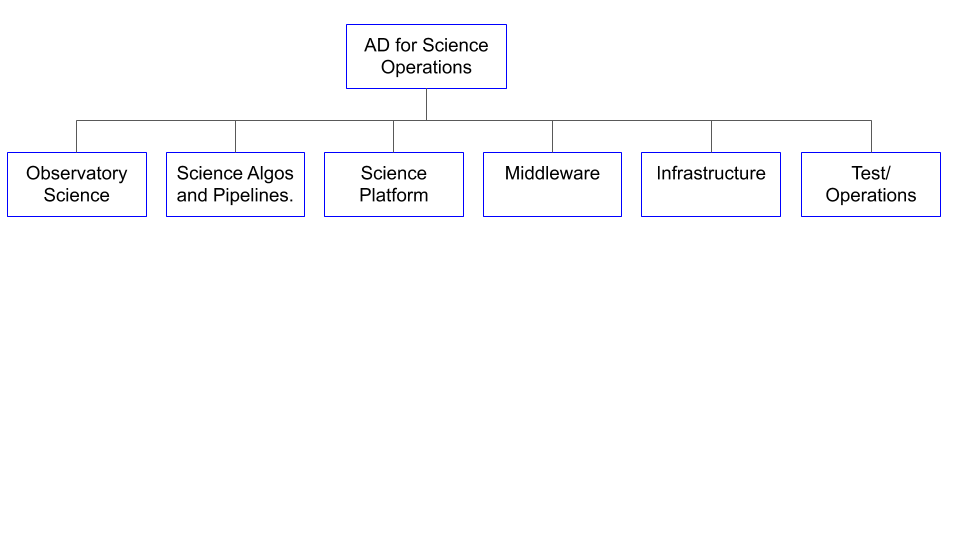
\includegraphics[width=0.9\textwidth]{figures/OrgOpsChart}
\caption{Possible configuration of Science Operations Department for operations of \gls{LSST} \label{fig:org}}
% original https://docs.google.com/presentation/d/1wIN6Dj_rPn8TASBUkAm6_-Yh255Gz9VbwFi61t4LCFs/edit#slide=id.g55f7c0247e_0_2
\end{figure}


\subsection{Other implied changes to the current operations proposal}
Notably missing from \figref{fig:org} is \gls{QA}. Currently \gls{QA} is spread across  three
 departments - the suggestion here is to place all \gls{QA} activities under the survey performance department. Consolidation
of the \gls{QA} activities in one department may allow for some personnel saving.

The data release team in science operations would require a verification scientist (this may be 0.5FTE) while the \gls{SDQA} and Semantic scientists may move to QA in survey science.

All data facility work, be it with a partner or in commercial \gls{cloud} should be firmly under science operations - hence there is no LDF department and no associate director for LDF.\footnote{This is  in line with AMCL recommendations}

